\documentclass[10pt]{article}
\usepackage{ctex}
\usepackage{graphicx}
\graphicspath{{E:/大学课程/大一下/人工智能程序设计/作业集/第十五周作业/图片集/},{pics/}}
\usepackage{amsmath}
\usepackage{amssymb}
\usepackage{float}%使图片紧跟在文字后面

\title{第十五周问答作业}
\author{朱士杭\ 231300027}
\date{\kaishu \today}

\begin{document}
	\maketitle
	
	\section{聚类的评价指标}
	聚类的评价指标主要分为内部评价指标与外部评价指标
	\subsection{内部评价指标}
	内部评价指标不需要外部参考模型,直接从聚类结果计算得出。
	比如现在有一个已经聚类好的结果,有若干个簇,设簇的中心点为ui,其中每个簇中心点之间的距离需要越远越好;
	每个簇内部的点集计算它们的离散程度,越密集越好
	\subsection{外部评价指标}
	外部评价指标需要参考模型,一般需要提供一个预期,然后计算$(xi,xj)$一共$n*(n-1)/2$个有序对的$SS,SD,DS,DD$的大小,
	即预测结果是否正确得到一个混淆矩阵,然后通过$a/(a+b+c)$计算Jaccard系数,通过与参考模型比较来评估聚类结果。
	
	\section{初始簇中心选择对聚类结果的影响}
	K-means聚类算法是一种迭代优化算法,将数据集划分为K个簇,使得每个数据点与其所属簇的中心点的距离之和最小。\par
	一般来说,初始簇中心的选择会对聚类结果又一些影响的
	(PPT上有一个聚类的例子就很好地说明了这一点,起始中心点的选择不同导致最后聚类结果有上下与左右的区别)\par
\subsection{收敛速度}初始中心的选择会影响算法的收敛速度。如果初始中心选得合适,可能只需要很少的迭代就能得到满意的聚类结果;
	反之,如果初始中心选择不当,可能需要更多的迭代才能收敛,或者甚至无法收敛到全局最优解。
	\subsection{局部最优}K-means算法容易陷入局部最优解。不同的初始中心可能会导致算法收敛到不同的局部最优解,这些解的质量可能相差很大。
	\subsection{聚类质量}初始中心的选择直接影响最终的聚类质量。不当的初始中心可能导致某些簇包含的数据点过少,或者某些数据点被错误地划分到其他簇中。
	\subsection{算法稳定性}如果初始中心随机选择,可能会导致算法结果的不稳定。即使是同一数据集,不同的初始中心可能会得到不同的聚类结果。
	
	
	\section{Apriori算法用于发现关联规则的基本原理}
	Apriori算法是一种用于频繁项集挖掘和关联规则学习的算法,
	基本原理是通过迭代识别数据集中的频繁项集,然后从频繁项集中提取强关联规则。
	
	\subsection{Apriori算法的基本思想}
	频繁项集:如果某个项集是频繁的,那么它的所有子集也是频繁的。
	反之,如果某个项集是非频繁的,那么包含该项集的所有超集也是非频繁的。(PPT上有)\par
	支持度:一个项集在所有交易中出现的频率称为支持度。支持度大于等于用户设定的最小支持度阈值的项集称为频繁项集。\par
	关联规则:关联规则由前件和后件组成,形如$A->B$\,
	关联规则的强度可以用支持度、置信度和提升度来衡量。
	置信度:说白了就是条件概率,就以A->B为例,置信度就是在A发生的条件下B发生的概率\par
	
	\subsection{如何通过剪枝提高效率}
	主要是在搜索树当中进行搜索的过程中,利用
	“某个项集是非频繁的,那么包含该项集的所有超集也是非频繁的”
	这个思想,用支持度去筛选,如果这个项集是非频繁的,那么就没有再往下继续搜索的必要了,直接剪枝即可\par
	并且将这个点拉入“黑名单”,之后在其他点进行搜索的过程中遇到“黑名单”中的点也直接剪枝就可以了\par
	这样的话这一棵搜索树只有n层(假设有n个点的话),再经过剪枝之后就可以把原先$2^n$的复杂度大大降低,极大地提高了效率
	
	
	
	\section{KNN算法进行异常检测(异常检测上课还没有讲)}
	在异常检测中,k-NN方法通过计算一个点与其邻近点的距离来评估该点的异常程度
	\subsection{KNN算法异常检测的步骤}
	首先选择近邻的数量,确定一个合适的k值,这个值取决于数据集的大小和特性。k值太小可能会导致模型对噪声敏感,k值太大可能会导致异常点被忽略。
	然后计算距离,对于数据集中的每个点,计算它与其它所有点的距离。常用的距离度量方法包括欧氏距离、曼哈顿距离和汉明距离等。
	再选择邻近点,对于每个点,根据计算出的距离找到最近的k个点。
	最后评估异常程度,一种方法是计算点到其k个最近邻的平均距离。如果一个点的平均距离远大于其他点,那么它可以被认为是异常点。\par
	另一种方法是基于密度,计算每个点的局部密度,然后根据密度阈值来判断是否为异常\par
	
	\subsection{还有哪些方法异常检测}
	不妨还可以使用层次聚类的方法,通过一层一层地进行聚类(这样就不用自己设置超参数k的值啦),
	然后取比较每个点离自己簇的中心点的距离,离得很远的点很有可能就是异常点\par
	还有一个自己思考后的结果,去计算每个点之间的距离(大不了计算$n*(n-1)/2$次),
	然后找出距离很大的那几个点缩小范围,然后再逐个进行检查
	
	\section{K-means算法对Iris数据集进行聚类}
	详情请见代码"K-means对iris数据集聚类.py"与"第十五周问答作业.ipynb"文件中聚类描述\par
	\subsection{评估聚类质量}
	\begin{figure}[H]
		\centering
		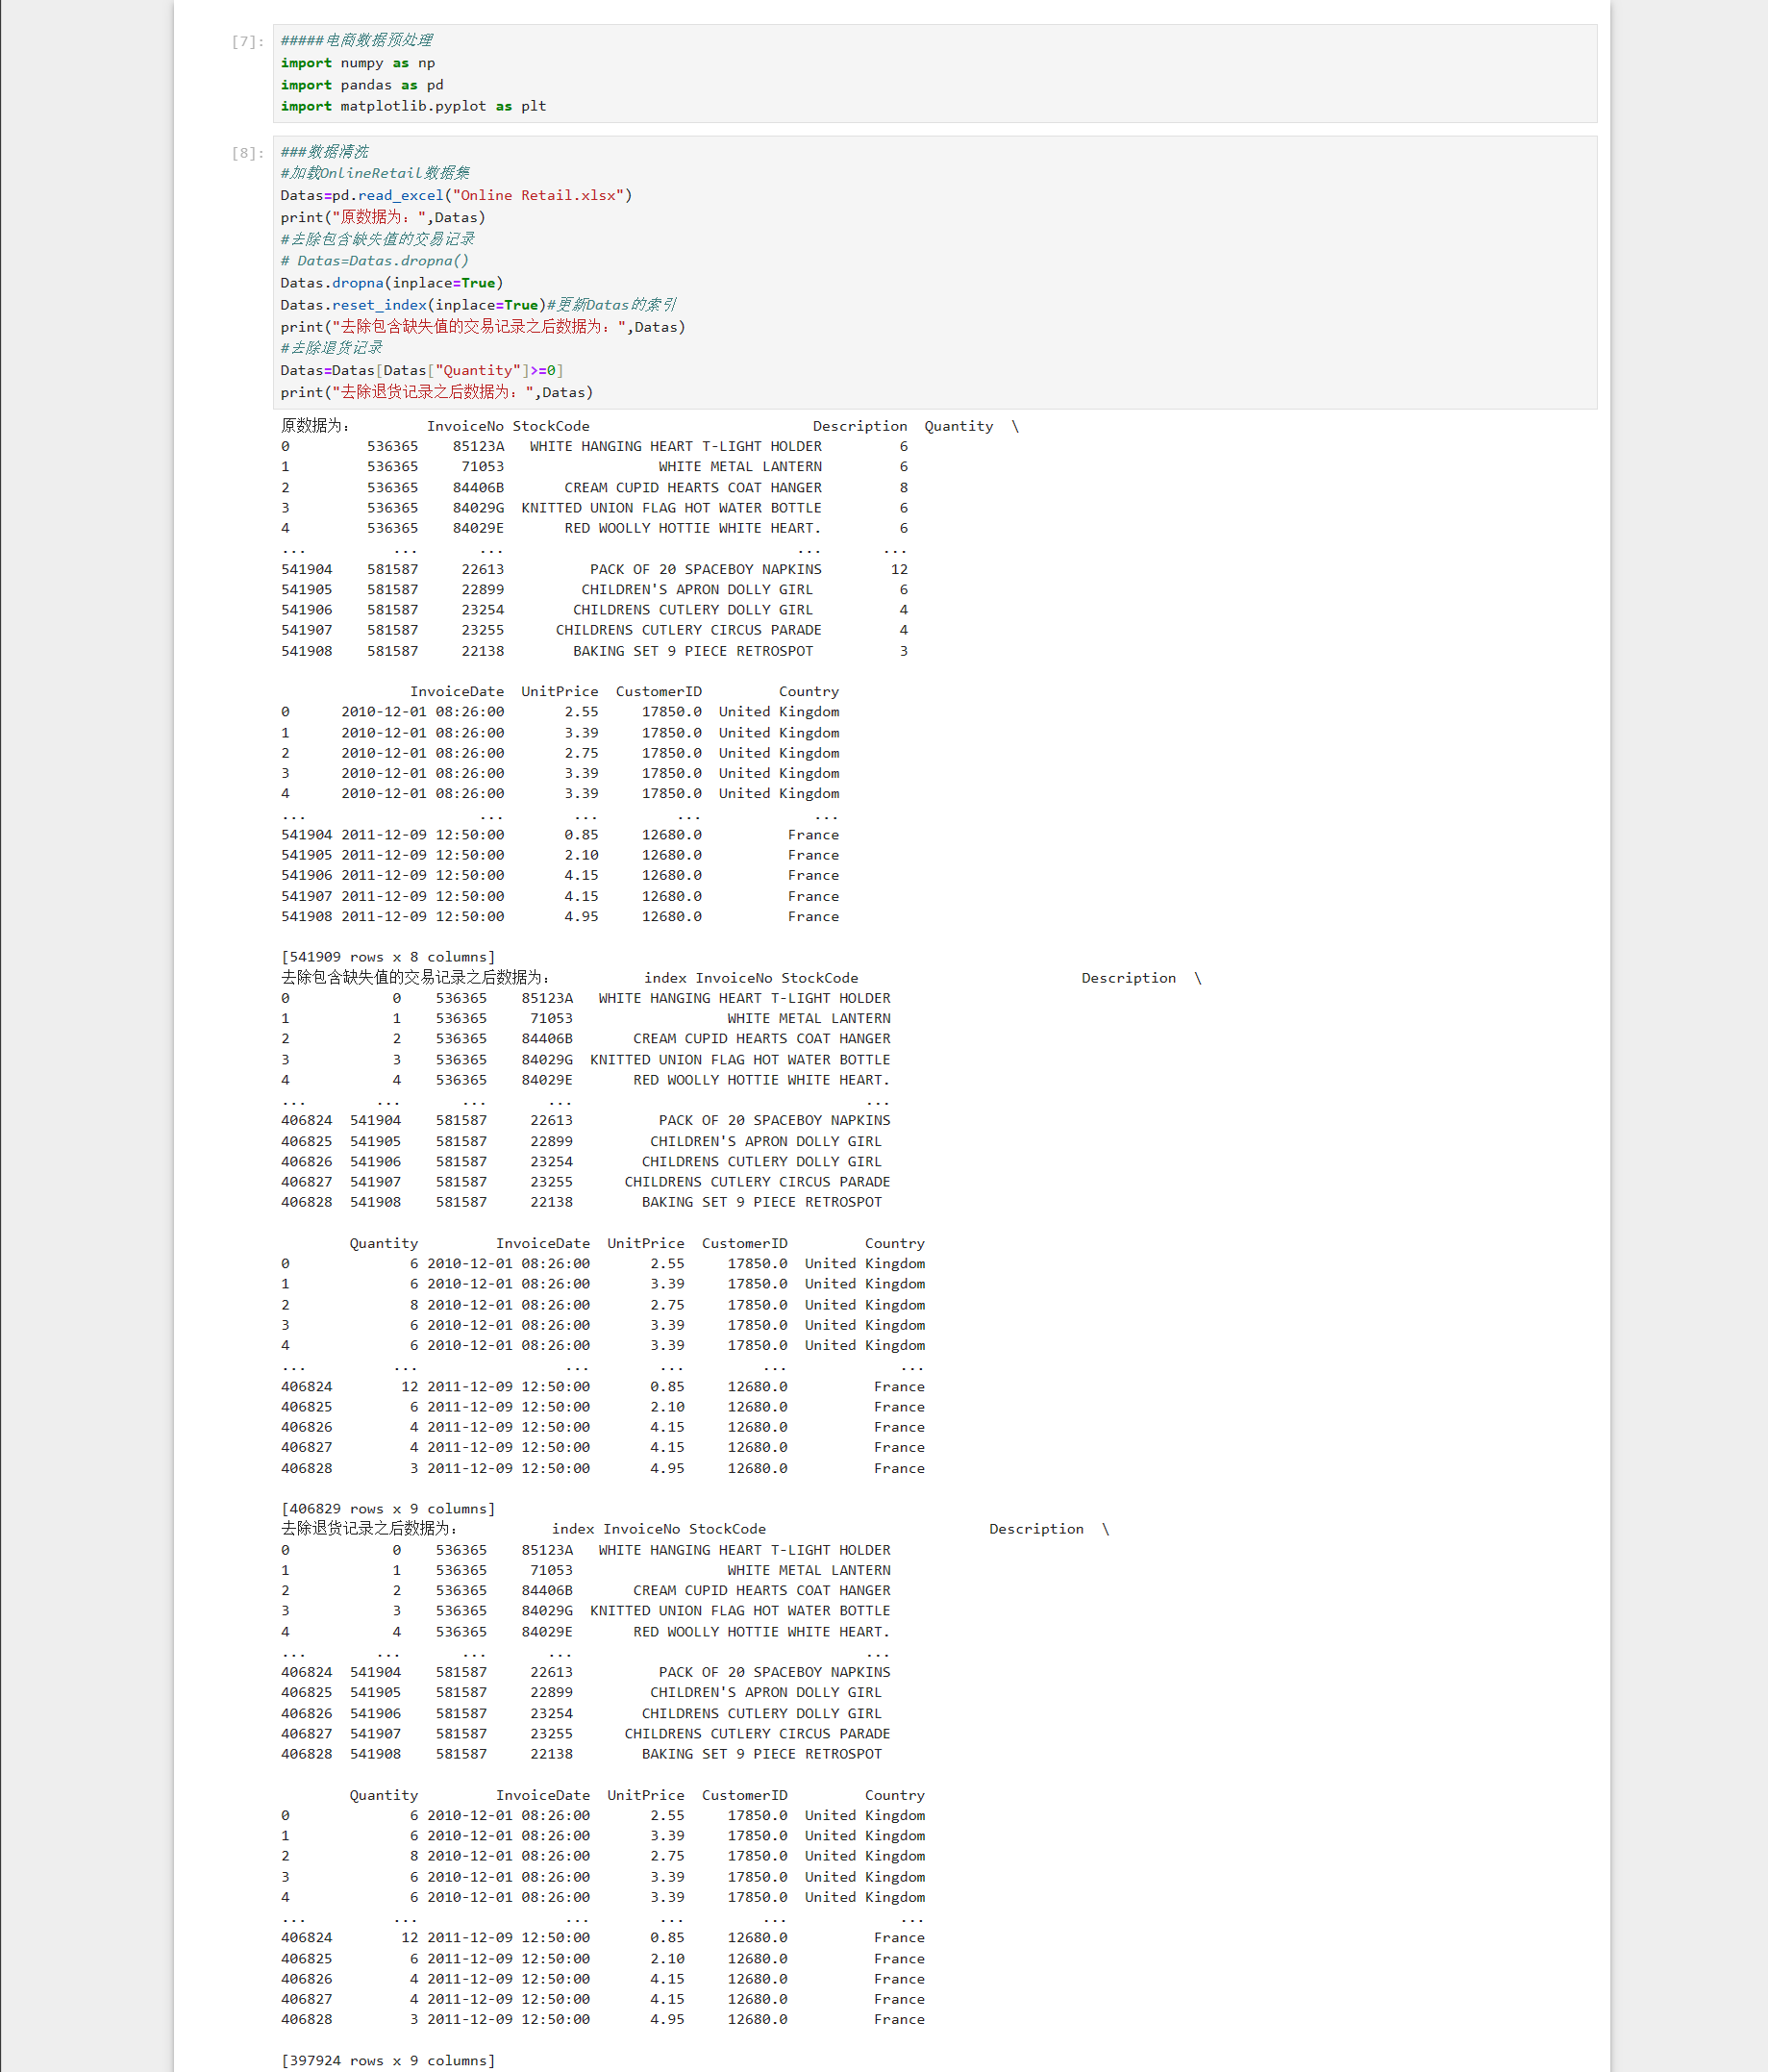
\includegraphics[scale=0.9]{1}
		\caption{聚类结果可视化}
	\end{figure}
	可见,聚类结果经过PCA之后效果很不错,能够将3个不同的类别自动区分,一开始设置的K值也是3,这个时候搭配得非常好\par
	
	\section{Apriori算法挖掘频繁项集,并生成关联规则}
	详情请见代码"K-Apriori算法生成OnlineRetail数据集关联规则.py"与"第十五周问答作业.ipynb"文件中对Apriori算法的相关描述\par
	算法结果就不贴了,代码写的一批吊糟,对于搜索树递归的相关知识完全忘了……之后有时间再补一补(至少没有调包全都是自己手写)
\end{document}